	%!TEX root = ../../Main.tex
\graphicspath{{Chapters/Krav/}}
%-------------------------------------------------------------------------------


\section{Krav}
I dette afsnit beskrives kravene til hvilken funktionalitet systemet har. 

\begin{itemize}
\item Systemet skal kunne finde de 4 stærkeste Bluetooth signaler. 
\item Systemet skal kunne køre uafbrudt
\item Systemet skal scanne efter Bluetooth enheder hvert 5. sekund i staten "LOCK AUTO".
\end{itemize}

\section{Aktørbeskrivelse}

\begin{figure}[H]
	\centering
	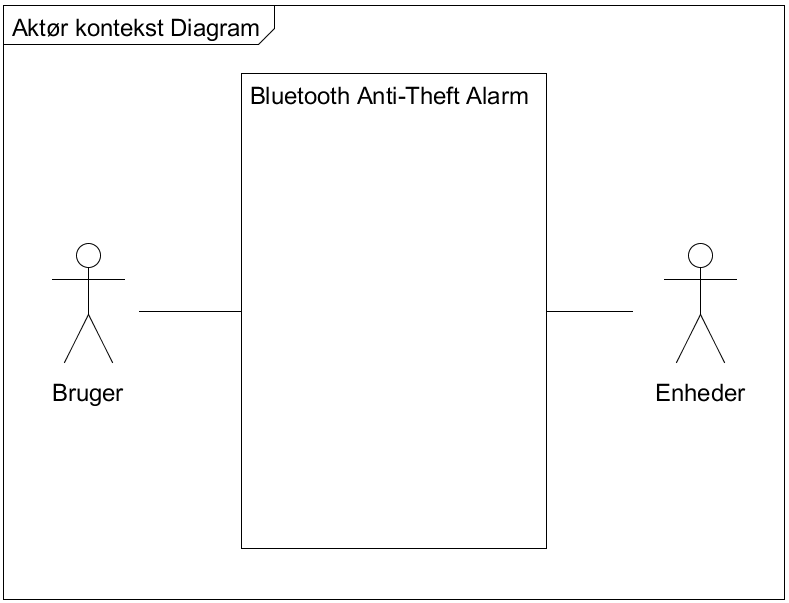
\includegraphics[width = 200 pt]{Img/Aktoer_Kontekst.png}
	\caption{Aktør kontekst diagram}
	\label{fig:Aktoer Kontekst diagram}
\end{figure}

På figur \ref{fig:Aktoer Kontekst diagram} ses aktør kontekst diagrammet som beskriver sammenhængen mellem aktørene og det system de interagere med. Aktørene er som følger: \\*
\begin{itemize}
\item \textbf{Bruger:} Aktøren der interagerer med systemet og dets funktionalitet \\
\item \textbf{BA-TA:} Bluetooth Anti-Theft Alarm systemet\\
\item \textbf{Enheder:} Op til 4 Bluetooth enheder som er registreret af BA-TA \\
\end{itemize}

\section{Use Case beskrivelse}

\begin{figure}[H]
	\centering
	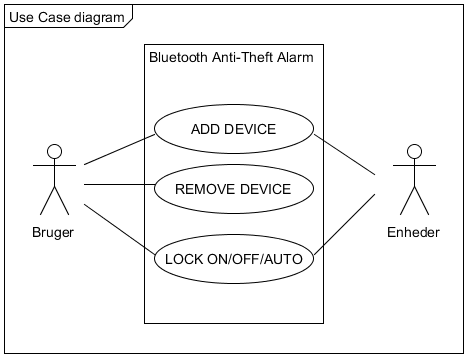
\includegraphics[width = 300 pt]{Img/Usecase_Diagram.png}
	\caption{Use Case diagram}
	\label{fig:Usecase diagram}
\end{figure}

På figur \ref{fig:Usecase diagram} ses usecase diagrammet som beskriver sammenhængen mellem aktørerne og de forskellige funktionaliteter der findes i systemet.

\subsection{UC 1 - ADD DEVICE}
\begin{itemize}
\item Brugeren trykker på "ENTER" når pilen er ved "ADD DEVICE".
\item Systemet scanner efter 4 stærkeste Bluetooth signaler.
\item Brugeren kan vælge imellem de registrerede Bluetooth-enheder, som skal tilføjes til listen over de godkendte enheder.
\end{itemize}


\subsection{UC 2 - REMOVE DEVICE}

\begin{itemize}
	\item Brugeren trykker på "ENTER" når pilen er ved "REMOVE DEVICE".
	\item Systemet præsenterer listen over de godkendte enheder.
	\item Brugeren kan vælge imellem de godkendte bluetooth-enheder, som brugeren ønsker at fjerne fra listen.
\end{itemize} 

\subsection{UC 3 - LOCK ON / LOCK OFF / LOCK AUTO}

\begin{itemize}
	\item Brugeren trykker på "ENTER" når pilen er ved "LOCK ON"/"LOCK OFF"/"LOCK AUTO".
	\item Systemet skifter state i rækkefølgen 1 - LOCK ON 2 - LOCK OFF 3 - LOCK AUTO.
\end{itemize}

%\section{Ikke-funktionelle krav}
%Kravene er delt op i tre underkategorier. Krav der relaterer til problemet. krav der relaterer til DSP platform og algoritme. Til sidst er der en kategori der beskriver kravene til systemet på baggrund af de to første kategorier.
%\begin{enumerate}
%	
%	\subsection{Problemrelateret krav}
%	\item R1: Systemet skal have 2 mikrofoner og 1 højtaler
%	
%	\item R2: Filteret skal gøre brug af LMS algoritmen
%	
%	\item R3: Systemet skal kunne processerer lyd i frekvensbåndet 50-20000Hz. 
%	
%	\item R4: Systemet skal kunne dæmpe uønkset støj 30dB.
%	
%	\item R5: Systemet skal kunne dæmpe støj uden at dæmpe ønsket lydsignal.
%	
%	\item R6: Systemet burde have en latency under 30ms.
%	
%	\item R7: Systemet burde have et dynamikområde på min 80dB
%	
%	\subsection{System og algoritme krav}
%	
%	\item R8: Filter algoritmen skal implementeres med fixed point 
%	
%	\item R9: Filteret skal max bruge 10kByte memory
%	
%	\item R10: Filteret skal implementeres på Blackfin BF533
%	
%	\item R11: Filteret må max benytte 98\% DSP load
%
%	\subsection{Afledte krav}
%	
%	\item DR1: DSP systemet skal kunne håndtere en samplingsrate på min 44100kHz(På baggrund af krav R3) 
%	
%	\item DR2: Filteret skal implementeres med 1.15 fixed point.(På baggrund af krav R7 og R8. Dette giver et dynamikområde på 96dB)
%	
%	\item DR3: Filter latency må max forsinkes 1280 samples(På baggrund af R6. (1/44100)*1280=30ms)
%	
%	\item DR4: Filteret må max bruge 13333 cycles af DSP processering for hver sample. (På baggrund af R10, R11 og DR1 (600MHz/44.1kHz)*98\%)
%	
%\end{enumerate}